\section{Data Preparation}
To prepare the data, we first defined selection criteria. We aimed to collect recitations from the best reciters worldwide to serve as references for judging Quran learners. In our study, we considered only \textit{Hafs} riwayah (\arb{رواية حفص}) as it's the most popular recitation method globally. Recognizing that manual data annotation requires significant effort and time, we created a 98\% automated pipeline for data collection. The steps are:
(1) Choose a digitized Quran script as the project foundation.
(2) Define criteria for \textit{Hafs} methodology.
(3) Collect expert recitations
(4) Segment recitations at pause points (\arb{وقف})
(5) Transcribe segments.
(6) Validate data through \textit{Tasmee} (\arb{تسميع}) Algorithm.
(7) Develop Quran Phonetic Script.

We define a \textit{Moshaf} as a complete Quran recitation (chapters 1-114) by a specific reciter. Statistics are summarized in table~\ref{tab:moshaf}. We manually annotated 5400 samples out of 286,537 utterances, resulting for the automation ratio of 98\%.

\begin{table}[htbp]
	\centering
	\caption{Dataset Statistics per Moshaf}
	\label{tab:moshaf}
	\begin{tabular}{ccc}
		\hline
		\textbf{Moshaf ID} & \textbf{Hours}       & \textbf{Length} \\
		\hline
		0.0                & 28.48          & 9133            \\
		0.1                & 40.31          & 10764           \\
		0.2                & 49.47          & 9971            \\
		0.3                & 37.19          & 12604           \\
		1.0                & 28.41          & 10939           \\
		2.0                & 51.05          & 9942            \\
		2.1                & 30.03          & 10394           \\
		3.0                & 25.19          & 10444           \\
		4.0                & 29.12          & 10994           \\
		5.0                & 28.02          & 11482           \\
		6.0                & 39.39          & 12435           \\
		7.0                & 28.26          & 9907            \\
		8.0                & 30.86          & 10330           \\
		9.0                & 27.95          & 10642           \\
		11.0               & 24.01          & 10363           \\
		12.0               & 33.42          & 9880            \\
		13.0               & 33.99          & 9377            \\
		19.0               & 30.11          & 11278           \\
		22.0               & 28.11          & 10332           \\
		24.0               & 28.51          & 9868            \\
		25.0               & 16.93          & 7922            \\
		26.0               & 30.44          & 11565           \\
		26.1               & 32.71          & 11850           \\
		27.0               & 28.05          & 11213           \\
		28.0               & 31.05          & 10535           \\
		29.0               & 27.79          & 11061           \\
		30.0               & 29.14          & 11312           \\
		\hline
		\textbf{Total}     & \textbf{847.9944402} & \textbf{286537} \\
		\hline
	\end{tabular}
\end{table}

\subsection{Choose a Digitized Version of the Holy Quran}
The Quran has multiple digitized versions including Tanzil\footnote{\url{https://tanzil.net}} and King Fahd Complex\footnote{\url{https://qurancomplex.gov.sa}}. We chose Tanzil because:
\begin{itemize}
	\item It uses standard Unicode characters
	\item Contains both \textit{Imlaei} and \textit{Uthmani} versions
	\item Maintains high accuracy
\end{itemize}
We excluded KFGQPC due to its evolving/unstable nature compared to Tanzil.

\subsection{Define Variant Criteria for Hafs}
\textit{Hafs} riwayah contains variants, e.g., \textit{Madd Al-Munfasil} (\arb{مد المنفصل}) can extend 2, 4, 5, or 6 beats. We rigorously defined these variants through the Qira'at literature \cite{al-dabbaa}, summarized in the following attributes in the Appendix section \ref{sec:moshaf_attributes}.


\subsection{Collect Expert Recitations}
We collected recitations from 22 world-class reciters with premium audio quality, totaling \textbf{893 hours} pre-filtering.

\begin{figure}[htbp]
	\centering
	\includegraphics[width=0.8\linewidth]{figures/stats.png}
	\caption{Database Collection Statistics}
	\label{fig:stats}
\end{figure}

\begin{figure}[htbp]
	\centering
	\includegraphics[width=0.8\linewidth]{figures/reciter.png}
	\caption{Reciters Statistics}
	\label{fig:reciters}
\end{figure}

We developed a web GUI using Streamlit\footnote{\url{https://streamlit.io/}} that:
\begin{itemize}
	\item Downloads and extracts metadata for each track
	\item Organizes data by Moshaf (each chapter as "001.mp3")
	\item Annotates Moshaf attributes
\end{itemize}

\subsection{Segment Recitations}
Since Tajweed rules are affected by pauses (\arb{وقف}), accurate segmentation is crucial. We initially tested open-source Voice Activity Detection (VAD) models including SileroVAD \cite{SileroVAD} and PyAnnotate \cite{Plaquet23}. Poor Quran-specific performance led us to develop a custom segmenter by fine-tuning Wav2Vec2-BERT \cite{barrault2023seamless} for frame-level classification.

\subsubsection{Preparing Segmenter Data}
We selected mosahf compatible with SileroVAD v4, using EveryAyah\footnote{\url{https://everyayah.com/}} (pre-segmented by ayah) as ground truth. After tuning parameters per Moshaf:
\begin{itemize}
	\item Threshold
	\item Minimum silence duration (merges segments)
	\item Minimum speech duration (discards short segments)
	\item Padding (added at segment boundaries)
\end{itemize}

\paragraph{Data Augmentation}
Using the Audiomentations \cite{Audiomentations} library, we replicated SileroVAD's noise setup on 40\% of samples, adding:
\begin{itemize}
	\item \texttt{TimeStretch} (0.8x-1.5x) to simulate recitation speeds
	\item Sliding window truncation (1-second windows) for long samples instead of exclusion
\end{itemize}

\subsubsection{Training Segmenter}
We fine-tuned Wav2Vec2-BERT for frame classification (1 epoch):

% \begin{figure}[htbp]
% \centering
% \includegraphics[width=\linewidth]{figures/vad-arch.png}
% \caption{VAD architecture vs. standard streaming models}
% \label{fig:vad-arch}
% \end{figure}

\begin{figure*}[b]
	\centering
	\includegraphics[width=0.85\textwidth]{figures/vad-arch.png}
	\caption{VAD architecture vs. standard streaming models}
	\label{fig:vad-arch}
\end{figure*}

Results of our segmenter on unseen mosahf in table~\ref{tab:seg_results}:

\begin{table}[htbp]
	\label{tab:seg_results}
	\centering
	\caption{Test results of the segmenter on unseen full moshaf. The result is validated by actual usage of the segmenter}
	\vspace{2pt}
	\begin{tabular}{lc}
		\hline
		\textbf{Metric} & \textbf{Value} \\
		\hline
		Test Loss       & 0.0277         \\
		Test Accuracy   & 0.9935         \\
		Test F1 Score   & 0.99476        \\
		\hline
	\end{tabular}
\end{table}

\subsection{Transcribe Segmented Parts}
We employed Tarteel ASR \cite{tarteel_whisper_ar_quran} (Whisper fine-tuned on Quranic recitations \cite{radford2023robust}). To handle its 30-second limit, we used sliding window truncation (10-second windows), with verification in the next step.

\subsection{Verification of Segmentation and Transcription}
\textbf{Segmentation Verification}: Manual inspection of 50-75 random samples per Moshaf. Moshaf 25.0 was excluded due to poor segmentation.

\textbf{Transcription Verification}: \textit{Tasmeea}-inspired algorithm:
(1) Match segments to Quranic text.
(2) Identify missing surah parts.
(3) Manual correction.

Refer to the Tasmeea Algorithm in the Appendix \ref{alg:tasmeea}

After matching, we catalogued missing Quranic portions per surah. Then correct transcription errors identified through the above process.

\begin{figure}[htbp]
	\centering
	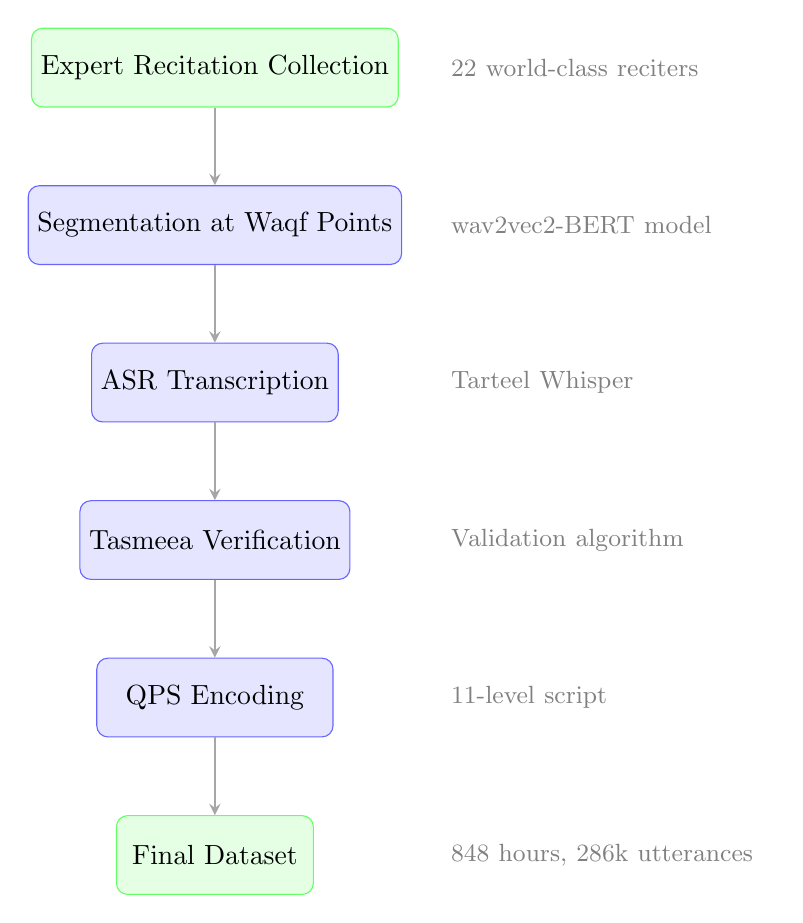
\begin{tikzpicture}[node distance=2cm, auto]
		% Define styles with simple colors
		\tikzstyle{process} = [rectangle, minimum width=3cm, minimum height=1cm, text centered, draw=blue!60, fill=blue!10, rounded corners]
		\tikzstyle{data} = [rectangle, minimum width=2.5cm, minimum height=1cm, text centered, draw=green!60, fill=green!10, rounded corners]
		\tikzstyle{arrow} = [thick,->,>=stealth,draw=gray!70]

		% Nodes
		\node[data] (collection) {Expert Recitation Collection};
		\node[process, below of=collection] (segmentation) {Segmentation at Waqf Points};
		\node[process, below of=segmentation] (transcription) {ASR Transcription};
		\node[process, below of=transcription] (verification) {Tasmeea Verification};
		\node[process, below of=verification] (encoding) {QPS Encoding};
		\node[data, below of=encoding] (dataset) {Final Dataset};

		% Arrows
		\draw[arrow] (collection) -- (segmentation);
		\draw[arrow] (segmentation) -- (transcription);
		\draw[arrow] (transcription) -- (verification);
		\draw[arrow] (verification) -- (encoding);
		\draw[arrow] (encoding) -- (dataset);

		% Side annotations
		\node[right of=collection, xshift=3cm, text width=4cm, text=gray] {\small 22 world-class reciters};
		\node[right of=segmentation, xshift=3cm, text width=4cm, text=gray] {\small wav2vec2-BERT model};
		\node[right of=transcription, xshift=3cm, text width=4cm, text=gray] {\small Tarteel Whisper};
		\node[right of=verification, xshift=3cm, text width=4cm, text=gray] {\small Validation algorithm};
		\node[right of=encoding, xshift=3cm, text width=4cm, text=gray] {\small 11-level script};
		\node[right of=dataset, xshift=3cm, text width=4cm, text=gray] {\small 848 hours, 286k utterances};
	\end{tikzpicture}
	\caption{The complete data preparation pipeline showing the six main stages from expert recitation collection to the final dataset generation. Each stage utilizes specialized models and algorithms to ensure high-quality annotations.}
	\label{fig:data_pipeline}
\end{figure}


